\documentclass[11pt, oneside]{article} 
\usepackage{geometry}
\geometry{letterpaper} 
\usepackage{graphicx}
	
\usepackage{amssymb}
\usepackage{amsmath}
\usepackage{parskip}
\usepackage{color}
\usepackage{hyperref}

\graphicspath{{/Users/telliott/Github/figures/}}
% \begin{center} \includegraphics [scale=0.4] {gauss3.png} \end{center}

\title{Heron and Brahmagupta}
\date{}

\begin{document}
\maketitle
\Large
Heron (or Hero) of Alexandria lived in the first century AD.  He was primarily an engineer, but is also remembered for Heron's Formula, which can be used to compute the area of a triangle from the lengths of its sides.  It is a simple formula that does not explicitly include the altitude $h$ or the parts of side $c$.

Heron's formula was later found to be a special case of a similar formula for quadrilaterals, discovered by Brahmagupta.

\begin{center}
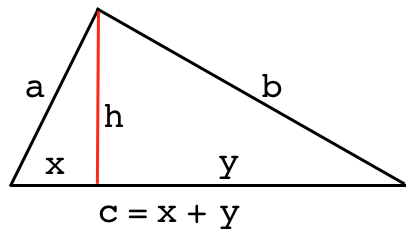
\includegraphics [scale=0.4] {triangle3.png}
\end{center}

If $s$ is one-half the perimeter, called the semi-perimeter, then
\[ 2s = a + b + c \]
then
\[ A = \sqrt{s \cdot (s-a) \cdot (s-b) \cdot (s-c)} \]

Proof.

From Lockhart.

\begin{center} 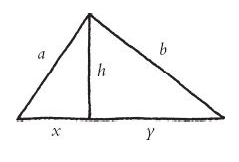
\includegraphics [scale=0.5] {triangle2.png} \end{center}

Side $c$ is split into $x$ and $y$.  We can write three equations:

\[ x^2 + h^2 = a^2 \]
\[ y^2 + h^2 = b^2 \]
\[ x + y = c \]

Our objective is an equation that contains only $a$, $b$ and $c$.  From the first two:
\[ a^2 - b^2 = x^2 - y^2 \]
and from the third:
\[ y^2 = c^2 - 2xc + x^2 \]
so
\[ a^2 - b^2 = x^2 - c^2 + 2xc - x^2 \]
\[ = 2xc - c^2 \]
then
\[ a^2 + c^2 - b^2 = 2xc \]

Finally a slight rearrangement:
\[ x = \frac{c^2 + a^2-b^2}{2c} = \frac{c}{2} + \frac{a^2-b^2}{2c}   \]

This says that to find the point where $c$ is divided into $x$ and $y$, we move from the center $c/2$ a distance of $(a^2 - b^2)/2c$.

The corresponding equation for $y$ is
\[ y = \frac{c}{2} - \frac{a^2-b^2}{2c} \]
which is easily checked by adding together the final two equations, obtaining $x + y = c$.

For the area, we will need $h$ somehow.  It is easier to use $h^2$.
\[ h^2 = a^2 - x^2 \]
\[ = a^2 - \frac{(c^2 + a^2-b^2)^2}{(2c)^2}  \]

The area squared is
\[ A^2 = \frac{1}{4}c^2 h^2 \]
\[ = \frac{1}{4} c^2 a^2 - \frac{1}{4} c^2 \frac{(c^2 + a^2-b^2)^2}{(2c)^2}  \]

Lockhart:

\begin{quote}
the algebraic form of this measurement is aesthetically unacceptable. First of all, it is not symmetrical; second, it's hideous. I simply refuse to believe that something as natural as the area of a triangle should depend on the sides in such an absurd way. It must be possible to rewrite this ridiculous expression...
\end{quote}

Here's a start:
\[ 16A^2 = (2ac)^2 - (c^2 + a^2-b^2)^2 \]

This is much better.  We immediately notice that it is a difference of squares.  First
\[ 16A^2 = \ [ \ 2ac + (c^2 + a^2-b^2) \ ] \ [ \ 2ac - (c^2 + a^2-b^2) \ ]  \]

But that has within it two squares, namely $(a + c)^2$ in the first term on the right-hand side, and $(a - c)^2$ in the second.

\[ 16A^2 = \ [ \ (a + c)^2 -b^2) \ ] \ [ \ b^2 - (a - c)^2 \ ]  \]
\[ 16A^2 =  (a + c + b)(a + c - b)(b + a - c)(b - a + c) \]

At this point, we recognize the semi-perimeter $2s = a + b + c$ and then we see that each of the other terms is $s$ minus one of the sides.  For example:
\[ a + c - b = 2s - 2b \]

So we obtain
\[ 16A^2 = 2s \cdot (2s - 2a) \cdot (2s - 2b) \cdot (2s - 2c) \]
\[ A^2 = s \cdot (s - a)(s - b)(s - c) \]

which you can of course write as the square root:
\[ A = \sqrt{s \cdot (s - a)(s - b)(s - c)} \]


\subsection*{check}
As a simple example, if we have a right triangle with sides 3,4,5, then the area is one-half of 3 times 4 = 6.  The semi-perimeter is s

\[ s = \frac{(3 + 4 + 5)}{2} = \frac{12}{2} = 6 \]
We have

\[ A =  \sqrt { 6 (6-5) (6-4) (6-3) } =  \sqrt { 6 (1) (2) (3) } = 6 \]

\subsection*{Brahmagupta}

Brahmagupta was an Indian mathematician who lived in the 7th century AD in a region of India called Bhinmal, which is in Rajastan.  He completed the square to obtain the quadratic equation, and did many other amazing things in trigonometry and arithmetic, as well as this example from geometry.

We consider a quadrilateral inscribed into a circle.  This is a special case, where the fourth point fits into the same circle determined by any three of the points.

\begin{center} 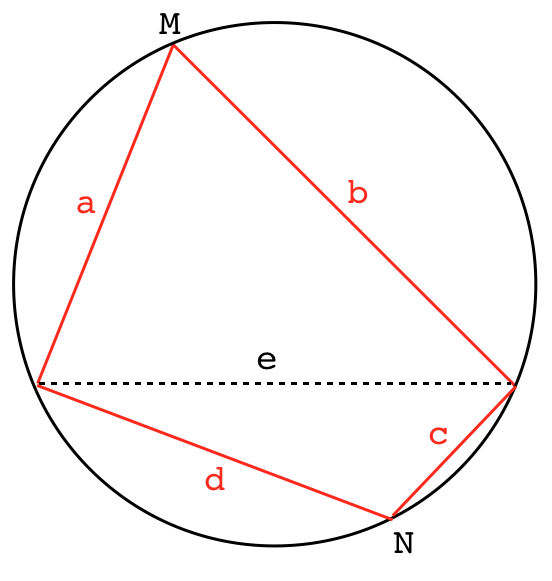
\includegraphics [scale=0.35] {brahmagupta.png} \end{center}

We will prove that the area of this quadrilateral is given by Brahmagupta's formula:

\[ A = \sqrt{(s-a) \cdot (s-b) \cdot (s-c) \cdot (s-d)} \]
Heron's formula is thus a special case where $d = 0$.
\[ A = \sqrt{s \cdot (s-a) \cdot (s-b) \cdot (s-c)} \]

\subsection*{preliminary}

We need two preliminary results.  If $M$ and $N$ are supplementary angles, then
\[ \sin M = \sin N, \ \ \ \ \ \ \cos M = - \cos N \]
(this becomes obvious if you plot them).

We also need the law of cosines (\hyperref[sec:Law_of_cosines]{\textbf{ref}}). 

Then, draw the line connecting the two opposing vertices which are not $M$ and $N$.  Using the law of cosines we can write two equal expressions for $e^2$, namely:
\[ e^2 = a^2 + b^2 - 2ab \cos M \]
\[ e^2 = c^2 + d^2 - 2cd \cos N = c^2 + d^2 + 2cd \cos M \]

Equating the two and grouping terms:
\[ a^2 + b^2 - c^2 - d^2 = 2(ab + cd) \cos M \]

Look at the diagram again.  

\begin{center} 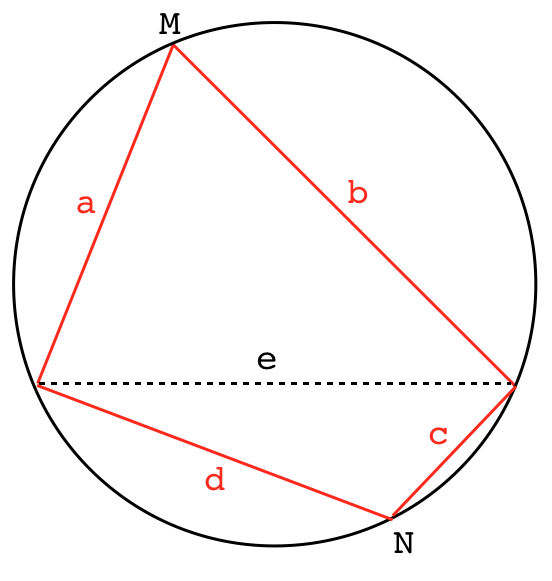
\includegraphics [scale=0.35] {brahmagupta.png} \end{center}

The triangle above the dotted line has area $(1/2) \ ab \sin M$ and similarly for the one below so the total area is
\[ A_1 = \frac{1}{2} ab \sin M \]
\[ A_2 = \frac{1}{2} cd \sin N = \frac{1}{2} cd \sin M \]

Adding, the total area is:
\[ A  =  \frac{1}{2}(ab + cd) \sin M \]
\[ 4A =  2(ab + cd) \sin M \]

\subsection*{algebra}

Square the two main equations so far:
\[ (a^2 + b^2 - c^2 - d^2)^2 =  \ [ \ 2(ab + cd) \ ]^2 \cos^2 M \]
\[ 16A^2 =  \ [ \ 2(ab + cd) \ ]^2 \sin^2 M \]
and add
\[ 16A^2 + (a^2 + b^2 - c^2 - d^2)^2 =   \ [ \ 2(ab + cd) \ ]^2 \]

Rearrange
\[ 16A^2 =   \ [ \ 2(ab + cd) \ ]^2 - (a^2 + b^2 - c^2 - d^2)^2 \]

As in Heron's derivation, we will proceed to factor two differences of squares.  

First:
\[ 16A^2 =   \ [ \ 2(ab + cd) + (a^2 + b^2 - c^2 - d^2) \ ] \ [ \ \ 2(ab + cd) - (a^2 + b^2 - c^2 - d^2) \ ] \]
\[ = \ [ \ (a + b)^2 - (c - d)^2 \ ] \  \ [ \ (c + d)^2 - (a - b)^2 \ ] \]
Second
\[ = (a + b + (c - d))(a + b - (c - d)) \ (c + d + (a - b))(c + d - (a - b)) \ ] \]
\[ = (a + b + c - d)(a + b - c + d)(c + d + a - b)(c + d - a + b) \]

If the semi-perimeter is $s$ then
\[ 2s = a + b + c + d \]

So we have
\[ 16A^2 = (2s - 2d)(2s - 2c)(2s - 2b)(2s - 2a) \]
\[ A^2 = (s - d)(s - c)(s - b)(s - a) \]

So lastly
\[ A^2 = (s - a)(s - b)(s - c)(s - d) \]
\[ A = \sqrt{(s - a)(s - b)(s - c)(s - d)} \]

\subsection*{comparison}

In comparing the two proofs, it's clear that Brahmagupta draws on the ideas of (i) using the semi-perimeter and (ii) difference of squares, which are in Heron's proof.  The main new idea is the law of cosines and the cancelation of $\sin^2 x + \cos^2 x$.

We can see this by rewriting the proof of Heron's formula in Brahmagupta's style.  First, the law of cosines.  Let $\alpha$ be the angle opposite side $a$:

\[ a^2 = b^2 + c^2 - 2bc \cos \alpha \]
\[ (b^2 + c^2 - a^2)^2 = (2bc)^2 \cos^2 \alpha \]

And the area is
\[ A = (1/2) bc \sin \alpha \]
\[ 4A = 2bc \sin \alpha \]
\[ 16A^2 = (2bc)^2 \sin^2 \alpha \]

Adding
\[ 16A^2 + (b^2 + c^2 - a^2)^2 = (2bc)^2  \]
\[ 16A^2 = (2bc)^2 - (b^2 + c^2 - a^2)^2  \]

This is what we had in the Lockhart derivation.  There is a slight difference because we have the term $(2bc)^2$ and we're subtracting $a^2$, but from the symmetry of the problem we know this is the same as having  $(2ac)^2$ and subtracting $b^2$.

The rest is exactly as before, it's just a matter of two differences of squares:
\[ 16A^2 = (2bc + (b^2 + c^2 - a^2))(2bc - (b^2 + c^2 - a^2)) \]
\[ = ((b + c)^2 - a^2) \ (a^2 - (b - c)^2) \]
\[ = (b + c + a)(b + c - a) \ (a + b - c)(a - b + c) \]

Involving the semiperimeter (and skipping over one step):
\[ A^2 = s(s - a)(s - b)(s - c) \]

$\square$




\end{document}